
% this file is called up by thesis.tex
% content in this file will be fed into the main document

% ----------------------- introduction file header -----------------------
\chapter{The LHC accelerator and the ATLAS experiment}
\label{chapter:ATLAS}
\begin{figure}[!h]
	\centering
	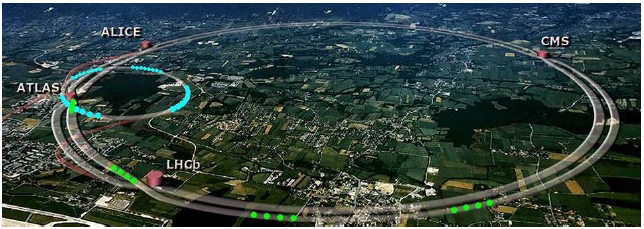
\includegraphics[width=0.885\textwidth]{Chapters/CH2/figures/CERN}
	\caption{The LHC ring, aerial view.}
	\label{fig:CERN}
\end{figure}
\noindent This chapter main focus is the experimental setup, thus the ATLAS detector, one of the four large experiments at CERN (\textit{Conseil Européen pour la Recherche Nucléaire}) and whose location is shown in Figure~\ref{fig:CERN}.\\\
Established in 1954, CERN is the largest particle physics laboratory in the world and the organization is based in a north-west suburb of Geneva on the Franco–Swiss border.
The analysis presented in this thesis is based on the data collected in Run2 (2015-2018).
Since December 2018, LHC has been shut-down (LS2, 2019-2020) to undergo a major upgrade (Phase \MakeUppercase{\romannumeral 1} Upgrade) which may enable to collect up to 300~$\mathrm{fb^{-1}}$ at a c.o.m. energy of 14~TeV by 2023. 
After that, a second major upgrade  (Phase \MakeUppercase{\romannumeral 2} Upgrade) is planned to the LHC (LS3, 2024-2025) which will increase the interaction rate by a factor of 10; this upgrade 
will lead LHC to High-Luminosity LHC (HL-LHC). 
% ----------------------- paths to graphics ------------------------

% the code below specifies where the figures are stored
\graphicspath{Chapters/CH2/figures}

% ----------------------------------------------------------------------
% ----------------------- introduction content -------------------------
% ----------------------------------------------------------------------

\section{The LHC accelerator}
Located at CERN, the Large Hadron Collider (LHC) ~\cite{CERN_acc} is the world’s highest energy particle accelerator.
LHC is a circular hadron accelerator, positioned at a depth of about 100~m in the tunnel built for the LEP accelerator.
It is 26.6~km long and currently operates by making proton beams collide at an energy $ \sqrt {s} = $ 13~TeV. \\
The overall accelerator complex is shown in Figure~\ref{fig:CERN_complex}.
\begin{figure}[!h]
	\centering
	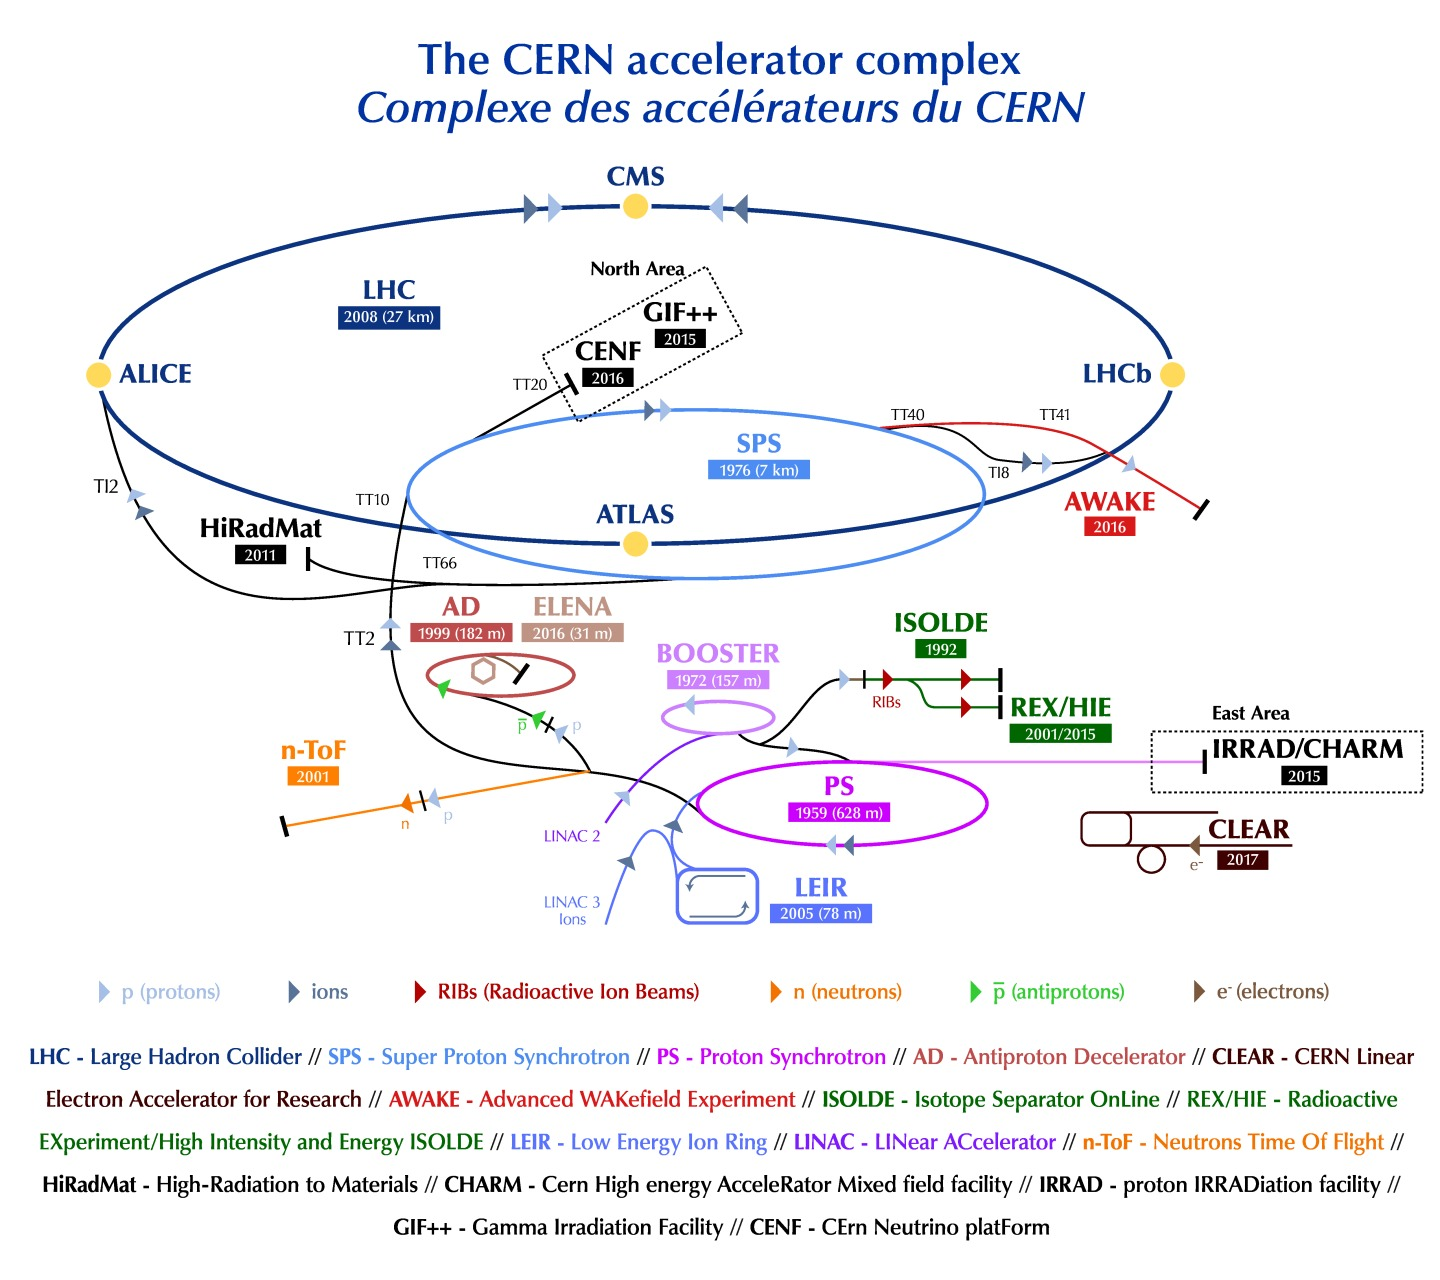
\includegraphics[width=0.97\textwidth]{Chapters/CH2/figures/CERN_complex}
	\caption{The overall CERN accelerator complex~\cite{CERN_complex}.}
	\label{fig:CERN_complex}
\end{figure}
\\CERN's choice to replace the LEP leptonic collider with an hadronic one, such as LHC, has brought two fundamental advantages: the first is that for the same infrastructural size it is possible to reach a higher energy in the center of mass, since the energy lost by radiation of synchrotron from a particle in circular motion is $\frac{dE}{dt}\propto\frac{E^4}{m^4R}$, where $R$ is the bending radius and $m$ is the mass of the accelerated particle travelling at an energy $E$, hence protons are better than electrons.
\newpage
\noindent The second advantage is that the composite structure of the protons allows access to a wider energy spectrum that can be explored simultaneously without having to change the beam parameters. On the other hand, the number of background events also increases.
In addition to proton-proton (p--p) collisions, the LHC can also collide heavy lead ions (Pb-Pb). \\
Before reaching the the target energy, protons undergo subsequent acceleration steps. \\
The first step is the proton production from hydrogen gas, after which protons are accelerated up to 50 MeV at the LINear ACcelerator 2 (LINAC 2). These protons are then injected into the 
Proton Synchrotron Booster (PSB) where their energy reaches 1.8~GeV.  The acceleration chain continues into the Proton Synchrotron (PS) which pushes the beam
to 25~GeV. After that, the beam is injected into the Super Proton Synchrotron (SPS) where the protons are accelerated up to 450~GeV. Finally, the bunches of protons are injected in the LHC.
A typical bunch train corresponds to 2808 bunches for each beam with 25~ns separation, and a bunch contains about $\mathrm{10^{11}}$ protons colliding at a rate up to 40~MHz. 
\\The LHC is designed to accelerate each beam at an energy of 7~TeV thanks to a complex system of dipole and higher order magnets but the LHC performance has not always been 
that of today. \\
The first protons beams were circulated in the LHC on September~\nth{10} of 2008. From 2010 to 2012, the protons
beams had an energy of 3.5~TeV. From 2012 to 2013, the energy reached was 4~TeV per beam. Following, the first shutdown, the LHC started to accelerate
beams up to an energy of 6.5~TeV in April~\nth{5} of 2015.\\
Since protons are charged particles, a strong magnetic field, produced by 1232 superconducting electromagnets, curves the beams around the circular accelerator.
To maintain the superconductivity properties, these magnets require a temperature of 1.9~K ($\mathrm{\approx}$271.3 \textdegree{}C). 
This temperature allows the dipole magnets to generate a magnetic field of 8~T. Besides the bending magnets, a total of 392 quadrupole magnets maintain the
beams focused and 16 radio-frequency cavities accelerate particles and keep them in controlled bunches with a constant energy.
Four main interaction points are used as collision points corresponding to the location of the four detectors: ALICE, ATLAS, CMS and LHCb.\\
%The beam in the LHC is not continuous but rather divided in a collection of protons (bunches) colliding at a rate up to 40 MHz. 
%The LHC beam at full intensity nominally consists of 2808 bunches and each bunch contains $\mathrm{\approx 1.15 \times10^{11}}$ protons, spaced by 25~ns.\\
The number of multiple interactions per bunch crossing is called \textit{pile-up} and it is denoted by $\mathrm{\mu}$. 
Actually there are two different sources of pile-up:
\begin{itemize}
	\item in-time pile-up occurs when multiple collisions take place in a single bunch crossing
	\item out-of-time pile-up is due to finite read-out time resolution of the detectors, often larger than 25 ns. In this case, the residual energy from
	a previous bunch crossing could potentially be associated to the following bunch crossing.
\end{itemize}
\newpage
\noindent The distribution of $\mathrm{<\mu>}$ is shown in Figure~\ref{fig:pileup}, for the different data-taking periods. The average pile-up for 2015-2018 is $\mathrm{<\mu>=33.7}$.
\begin{figure}[h]
	\centering
	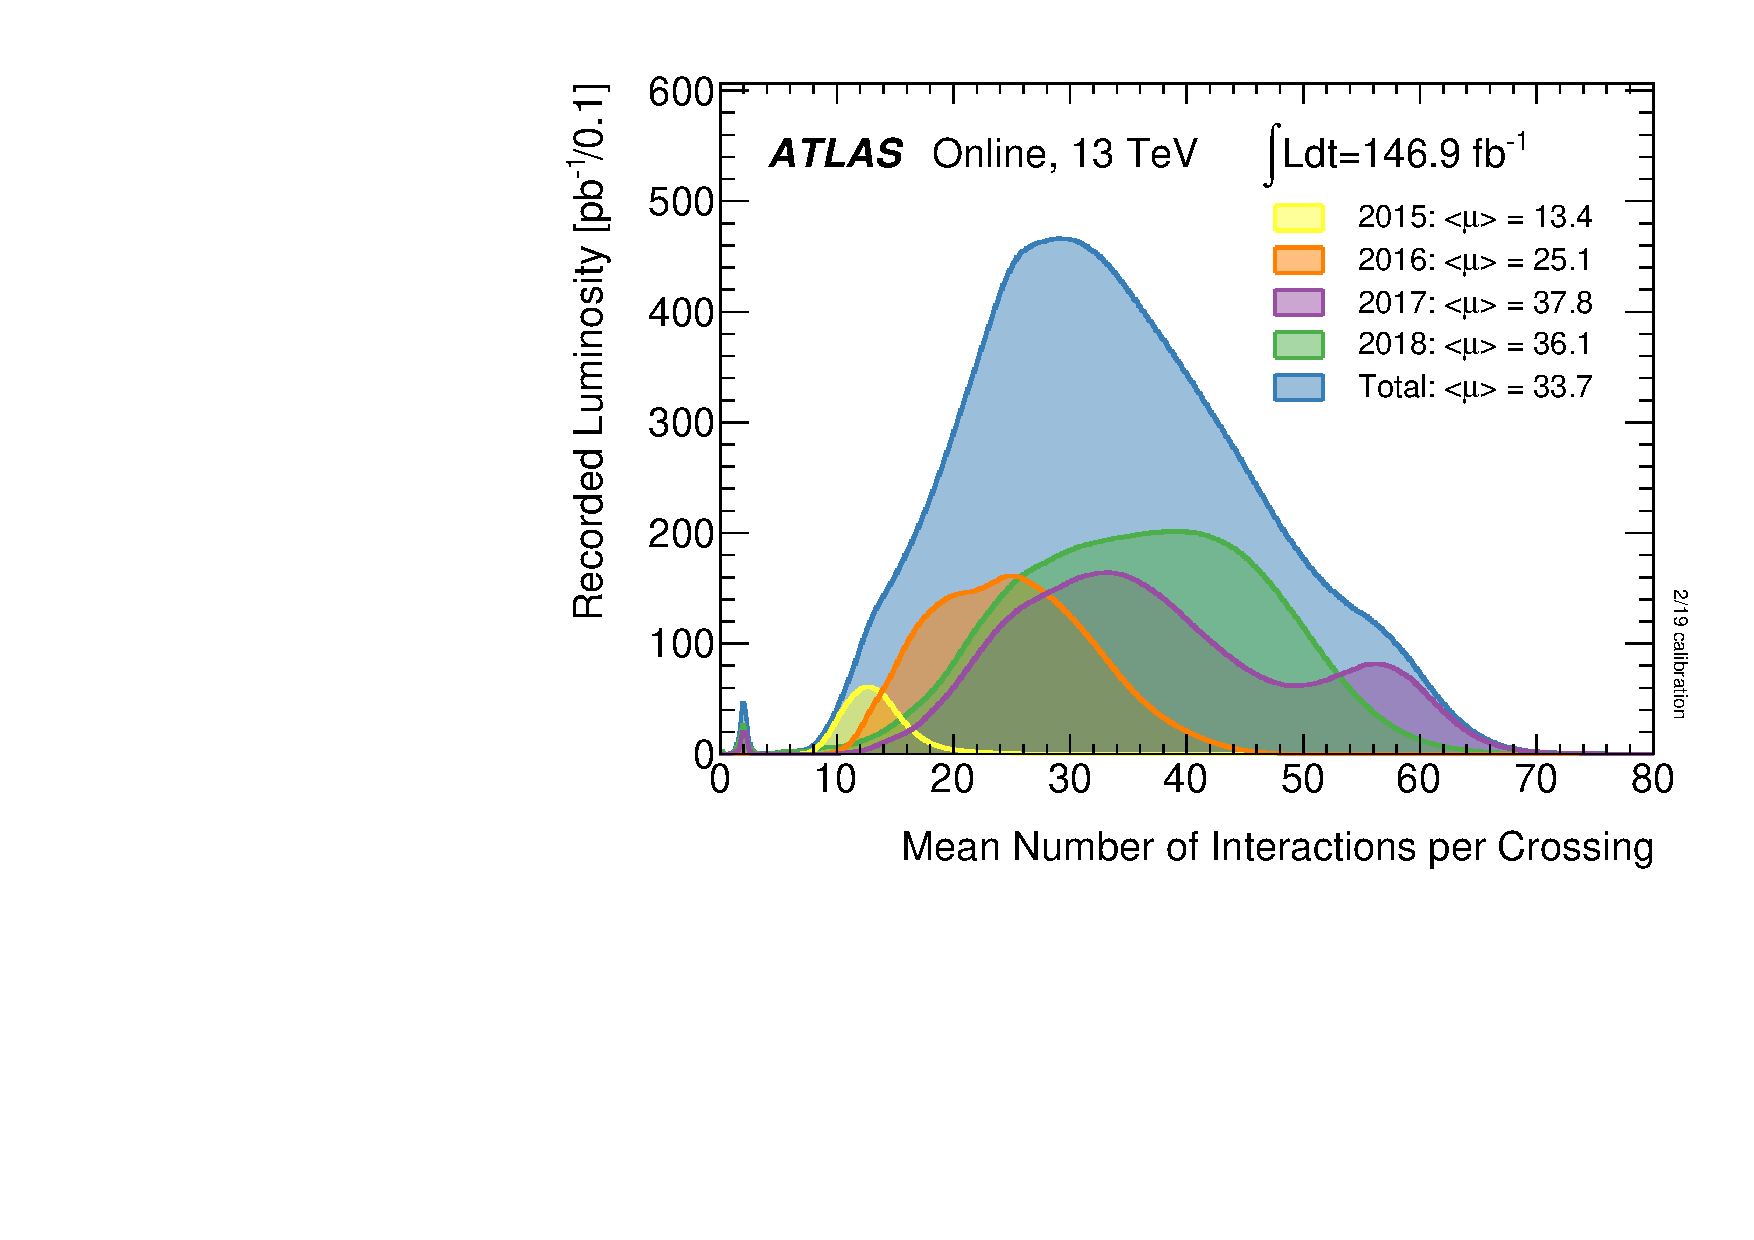
\includegraphics[width=100mm]{Chapters/CH2/figures/mu_2015_2018}
	\caption{Luminosity-weighted distribution of the mean number of interactions per crossing for the 2015-2018 pp collision data at $\mathrm{\sqrt{13}}$.  All data recorded by ATLAS during stable beams is shown, and the integrated luminosity and the mean mu value are given in the figure~\cite{lumi}.}
	\label{fig:pileup}
\end{figure}
\\The event rate of a given process with cross section $\sigma$ is given by $\frac{dN}{dt}=\mathcal{L} \sigma$, where $\mathcal{L}$ is 
a characteristic of the accelerator, known as \textit{instantaneous luminosity} and is given by:
\begin{equation}
\mathcal{L} =  \frac{N^{2}_{b}k_{b}f\gamma}{4\pi\sigma_{x}\sigma_{y}}F
\end{equation}
where $N^{2}_{b}$ is the number of particles per bunch, 
$k_{b}$ is the number of bunches, 
$\gamma$ represents the relativistic gamma factor, 
$f$ is the revolution frequency of the accelerator, 
$\sigma_{x}$ and $\sigma_{y}$ are the horizontal and vertical beam size, 
$F$ is a geometrical correction factor from the crossing-angle of the two beams at the interaction point (IP). 
\\Given a period of time T, one can define the \textit{integrated luminosity} as L= $\int^{T}_{0}{dt \mathcal{L}}$ 
which is typically expressed in $\mathrm{fb^{-1}}$ (1 $\mathrm{b = 10^{-28} m^{2}}$).
\\Figure~\ref{fig:lum} shows the total integrated luminosity over the full LHC data taking period at $\mathrm{\sqrt{13}}$ TeV and Table~\ref{tab:lum} summarizes the main design parameters of the LHC.
\begin{figure}[!ht]
	\centering
	\subfigure[]{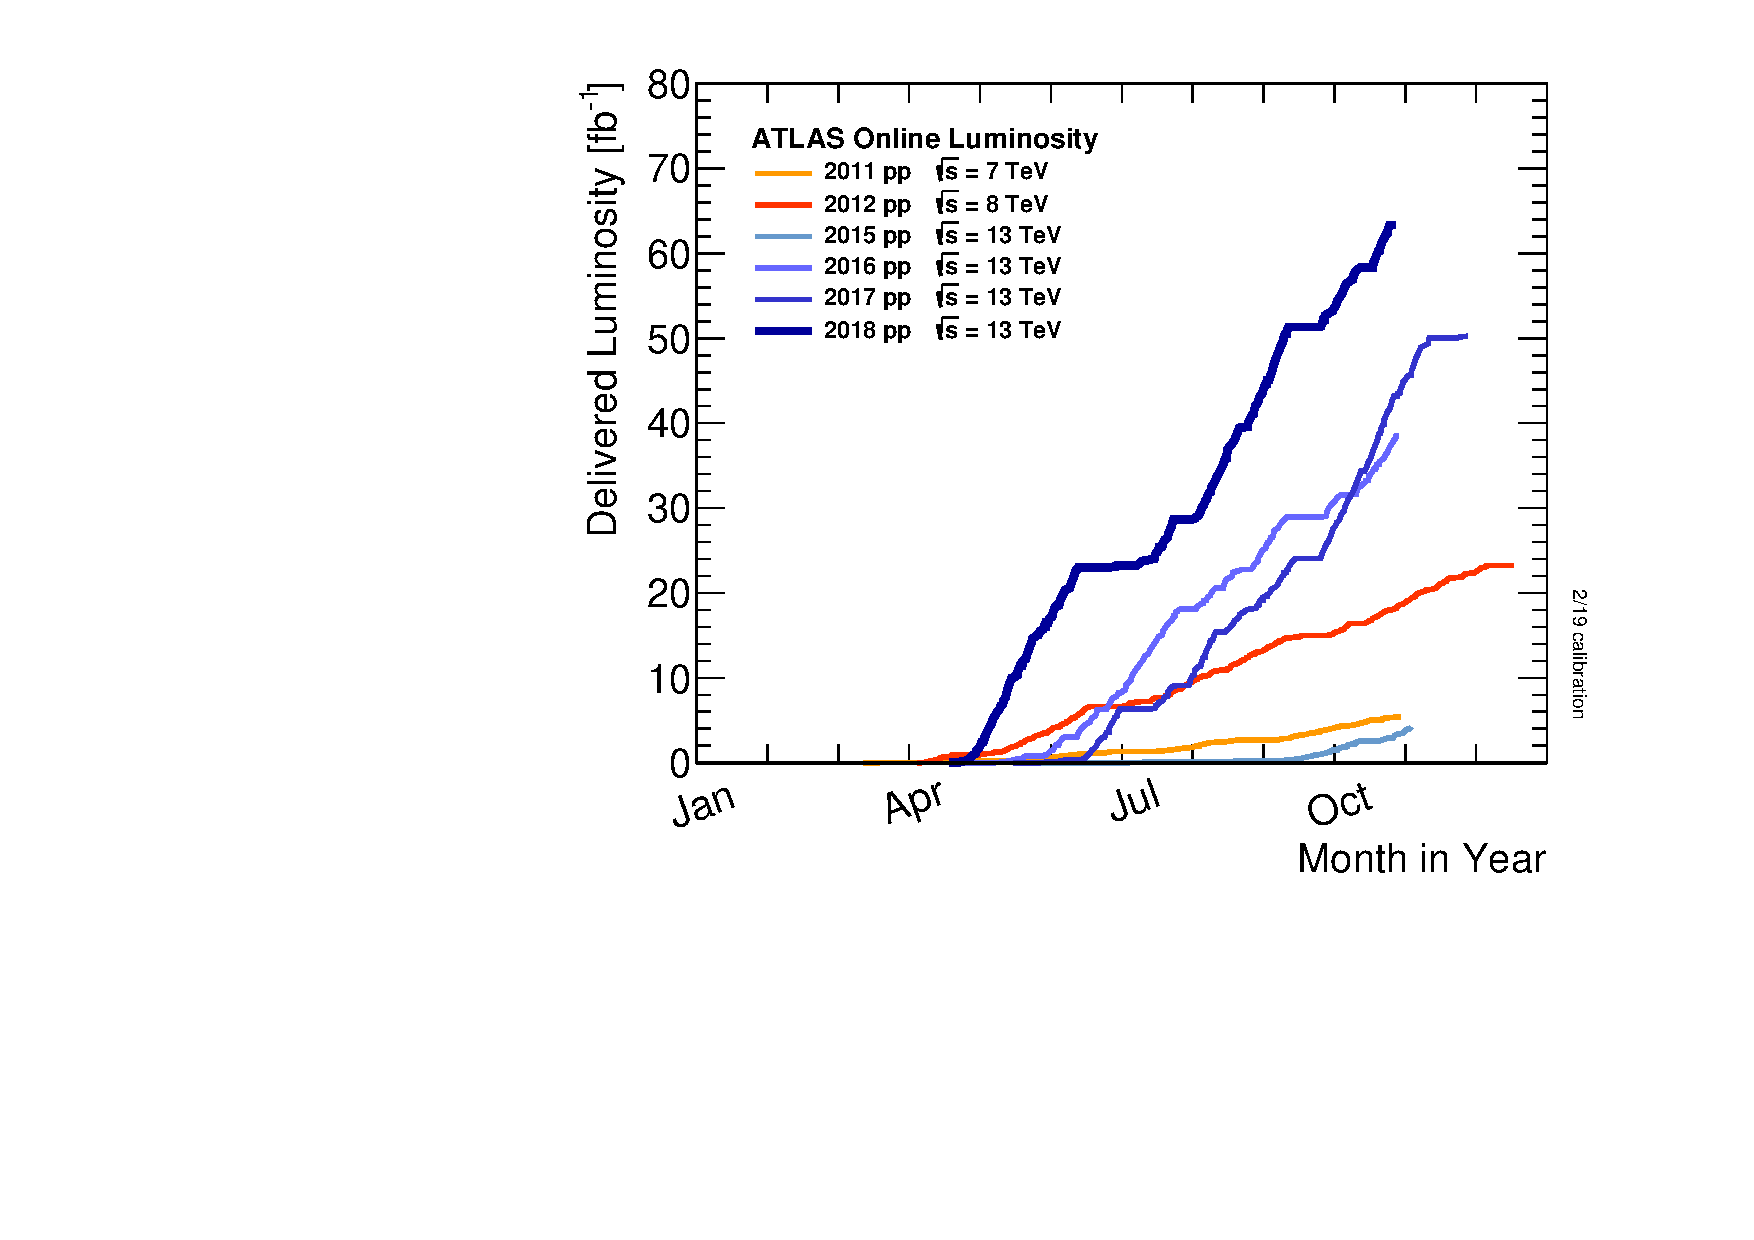
\includegraphics[width=75mm]{Chapters/CH2/figures/intlumivsyear}}\quad
	\subfigure[]{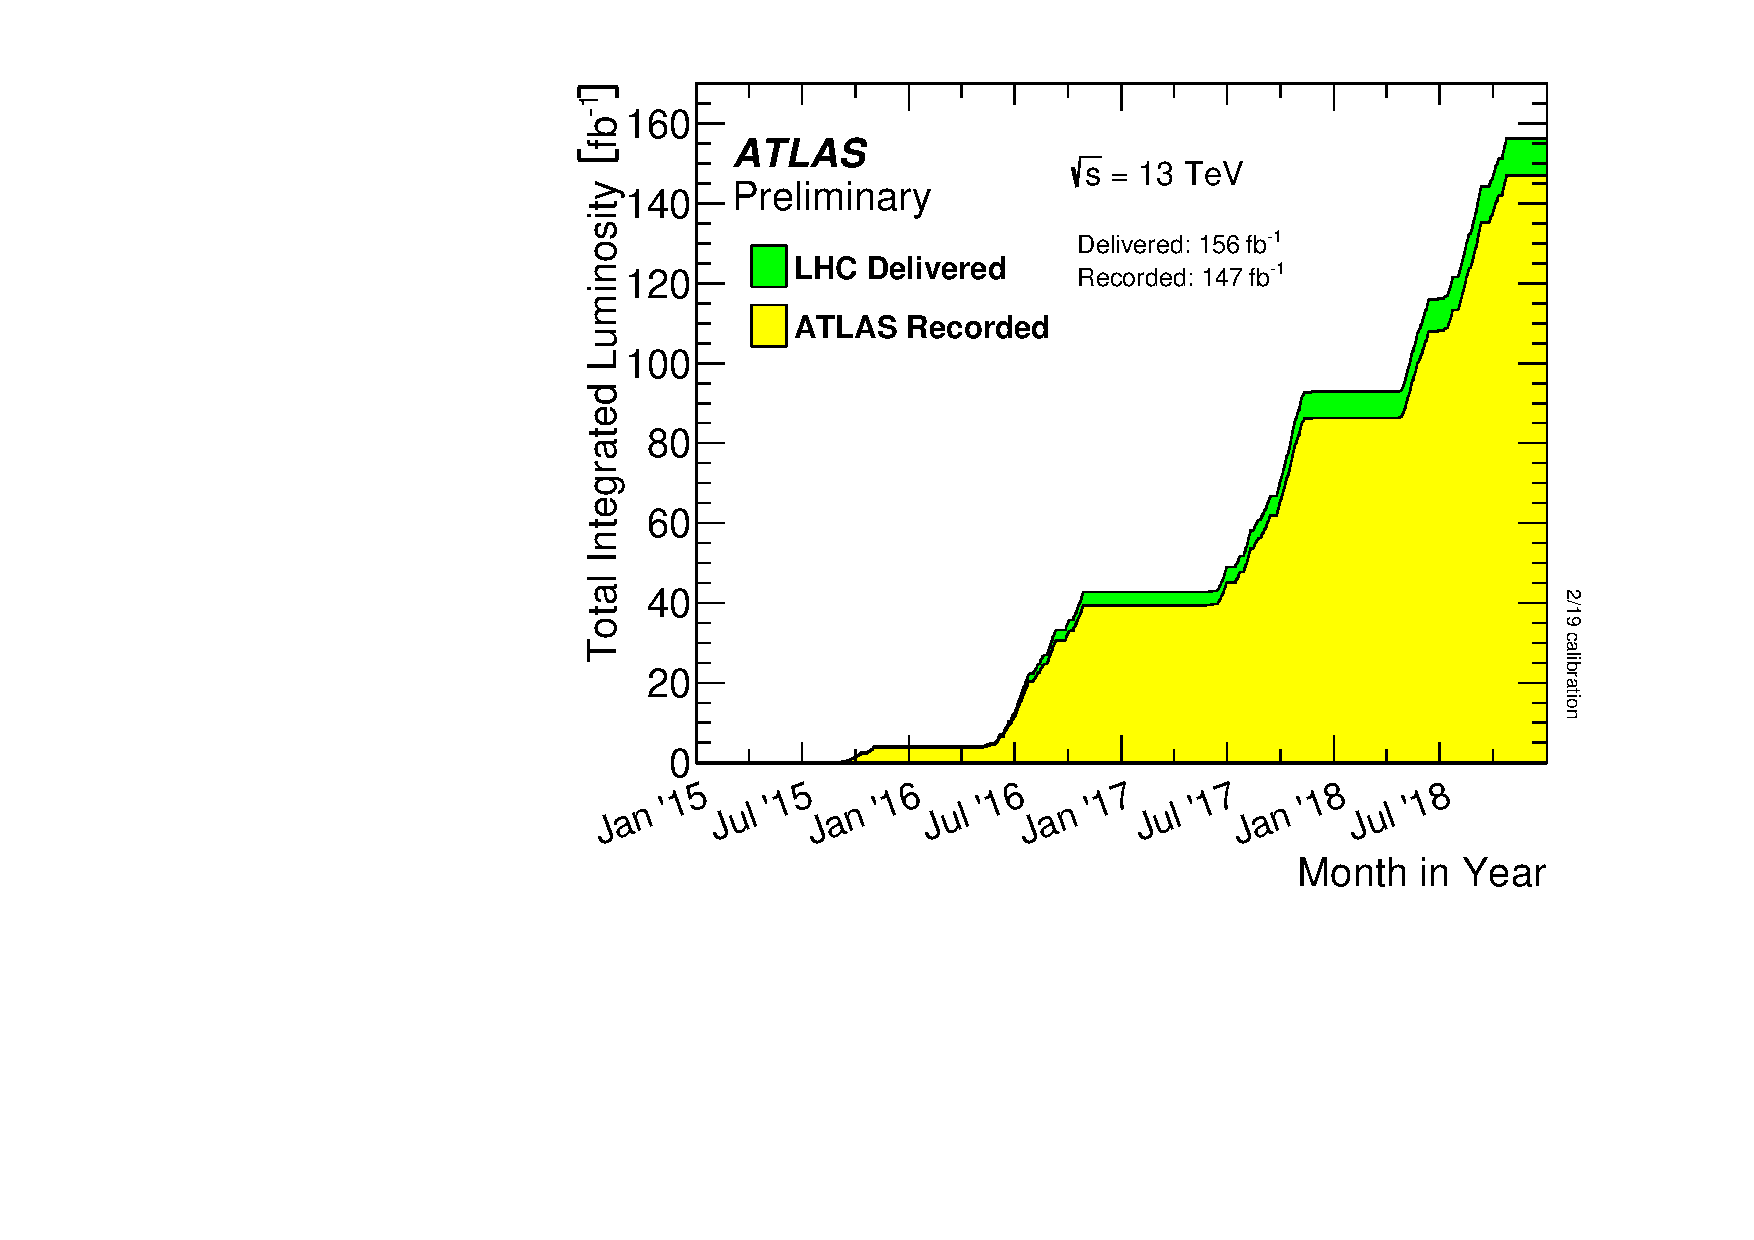
\includegraphics[width=75mm]{Chapters/CH2/figures/intlumivstimeRun2}}\quad
	\caption{Cumulative luminosity versus $a$) day delivered to ATLAS during stable beams; $b$) time delivered to ATLAS (green) and recorded by ATLAS (yellow) during stable beams for pp collisions at $\mathrm{\sqrt{13}}$~\cite{lumi}.}
	\label{fig:lum}
\end{figure}
\begin{table}[!h]
	\begin{adjustbox}{max width=1.\textwidth,center}
		\begin{tabular}{lcccc}
			\hline 
			\textbf{Parameter}              											&  \textbf{2015} & \textbf{2016} 			& \textbf{2017} & \textbf{2018} \\ 
			\hline 
				Bunch intensity [$\mathrm{\times10^{11}p}$] 		  &  1.2 				  & 1.1 						  & 1.25 				& 1.15 				\\
				Number of bunches   												 &  2200 			   & 2200						 & 1900				  & 2500			\\
				Emittance [$\mathrm{\mu m}$] 							 	  & 3.5					  & 2.5 						  &2.0 					 & 2.2				 \\
				Crossing angle [$\mathrm{\mu rad}$] 					   & 290 				  & 280 						 & 300 				   & 300		      \\
				Peak luminosity [$\mathrm{10^{34} cm^{2}s^{-1}}$] 	& 0.5 					& 1.5 							& 1.5				   &  2.0				\\
			\hline  
		\end{tabular} 
	\end{adjustbox}
	\caption{Main beam parameters of proton-proton collisions of LHC in Run2.}
	\label{tab:lum}
\end{table} 
\clearpage

\section{The ATLAS detector}
ATLAS (A Toroidal LHC ApparatuS)~\cite{ATLAS} is a multi-purpose apparatus whose primary goal is to identify and measure the properties of particles produced in p--p collision.\\
The overall ATLAS detector layout is shown in Figure~\ref{fig:ATLAS}.
The ATLAS detector consist of a concentric cylinder shape (4$\pi$ coverage), therefore nominally forward-backward symmetric with respect to the interaction point (IP) where the proton beams collide in it.
It can be divided into five main parts:
\begin{itemize}
	\item Magnet System (section~\ref{sec:MagSys});
	\item The Inner Detector  (section~\ref{sec:ID});
	\item The Calorimetric System  (section~\ref{sec:CAL});
	\item Muon Spectrometer  (section~\ref{sec:MuonSpec}).
	\item Trigger and data acquisition System  (section~\ref{sec:TrigSys}).
\end{itemize}
\begin{figure}[h]
	\centering
	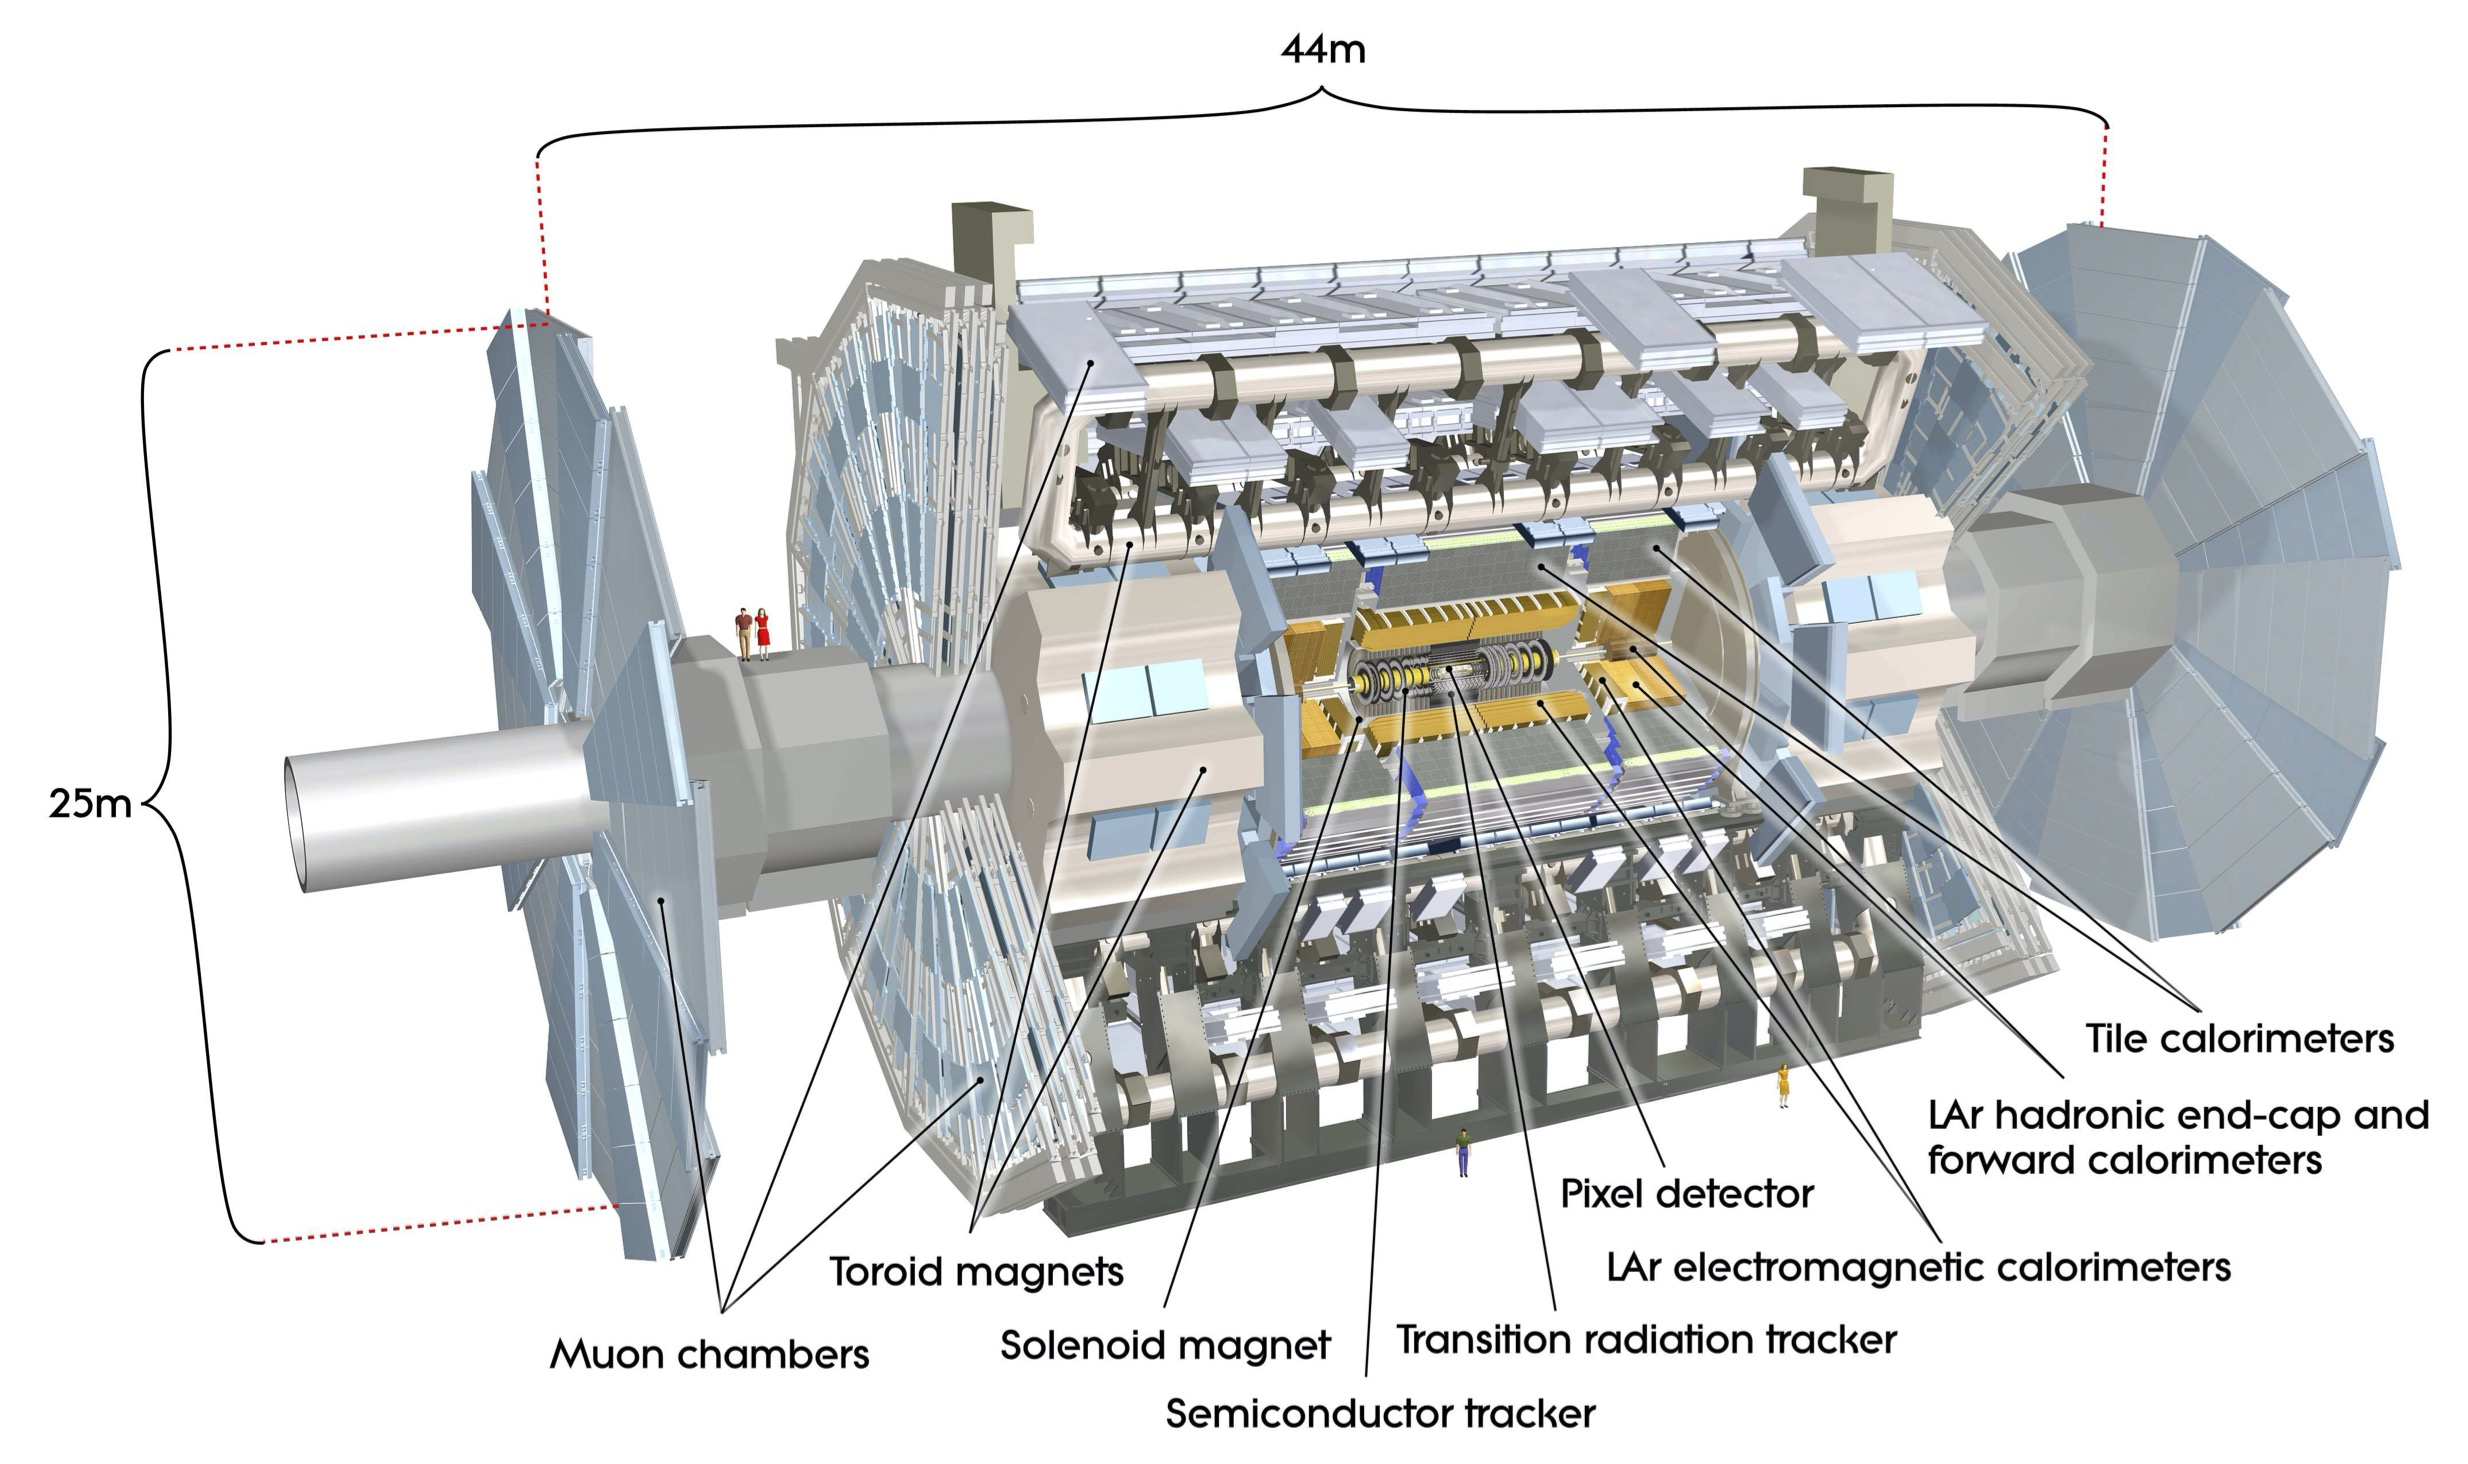
\includegraphics[width=110mm]{Chapters/CH2/figures/ATLAS}
	\caption{Cut-away view of the ATLAS detector. The dimensions of the detector are 25 m in height and 44 m in length. The overall weight of the detector is approximately 7000 tonnes~\cite{ATLAS}.}
	\label{fig:ATLAS}
\end{figure}
\clearpage
\subsubsection*{Coordinate system}
The ATLAS coordinate system is a right-handed Cartesian coordinate system with the origin defined at the IP, in the center of the detector.
The $z$-axis corresponds to the beam pipe while the $x$ and $y$ directions define the transverse plane.\\
A cylindrical coordinate system is often used due to the geometry of the detector, where $\phi$ is the azimuthal angle and $\theta$ is the polar angle. 
The $\phi$ is orthogonal to the beam direction, therefore it is invariant under a Lorentz boost($z$-axis), while $\theta$ is not an invariant, so the \textit{pseudorapidity} is defined as:
\begin{equation}
\eta=-\ln{(\tan{\bigg(\frac{\theta}{2}\bigg)})}
\end{equation}
Pseudorapidity is an approximation of the \textit{rapidity}\footnotemark for relativist particles ($m\ll p$) with mass $m$ and momentum $p$.
\footnotetext{Rapidity is defined as $y=\frac{1}{2}\ln{\frac{E+p_z}{E-p_z}}$}
\\The distance between two objects is indicated using $\mathrm{\Delta R}$, defined as:
\begin{equation}
\Delta R =\sqrt{\Delta \eta^{2}+\Delta \phi^{2}}
\end{equation}
The transverse momentum is the projection of the momentum orthogonal to the beam direction, defined as:
\begin{equation}
p_{T}=\sqrt{p^{2}_{x}+p^{2}_{y}}
\end{equation}

\subsection{Magnet System}
\label{sec:MagSys}
The magnet configuration comprises a thin superconducting solenoid surrounding the inner-detector cavity, and three large superconducting toroids (one barrel and two end-caps) arranged with an eight-fold azimuthal symmetry around the calorimeters. This fundamental choice has driven the design of the rest of the detector.\\
The inner detector is immersed in a 2 T solenoidal field provided by the central solenoid with inner radius of 1.23 m and a total length of 5.8 m.\\
It is designed to minimize the amount of material in front of the calorimeter to have a small impact on the energy measurement. This is achieved by hosting the solenoid and
the cryostat in the same vacuum vessel of the electromagnetic calorimeter.\\
The overall dimensions of the magnet system is 26 m long and 20 m diameter and provide and average magnetic field intensity of 0.5 T in the barrel and 1 T in the end-caps regions~\cite{MagSys}.
\clearpage
\subsection{Inner Detector}
\label{sec:ID}
The Inner Detector (ID)~\cite{ATLAS} is the detector system closest to the beam.\\
It is composed of three detectors: the semiconductor pixel detector (PIXEL), the microstrip detector SCT (Semi-Conductor Tracker), and the most external, the transition radiation detector TRT (Transition Radiation 
Tracker).\\
Its overall layout is depicted in Figure~\ref{fig:ID}.
\begin{figure}[h]
	\centering
	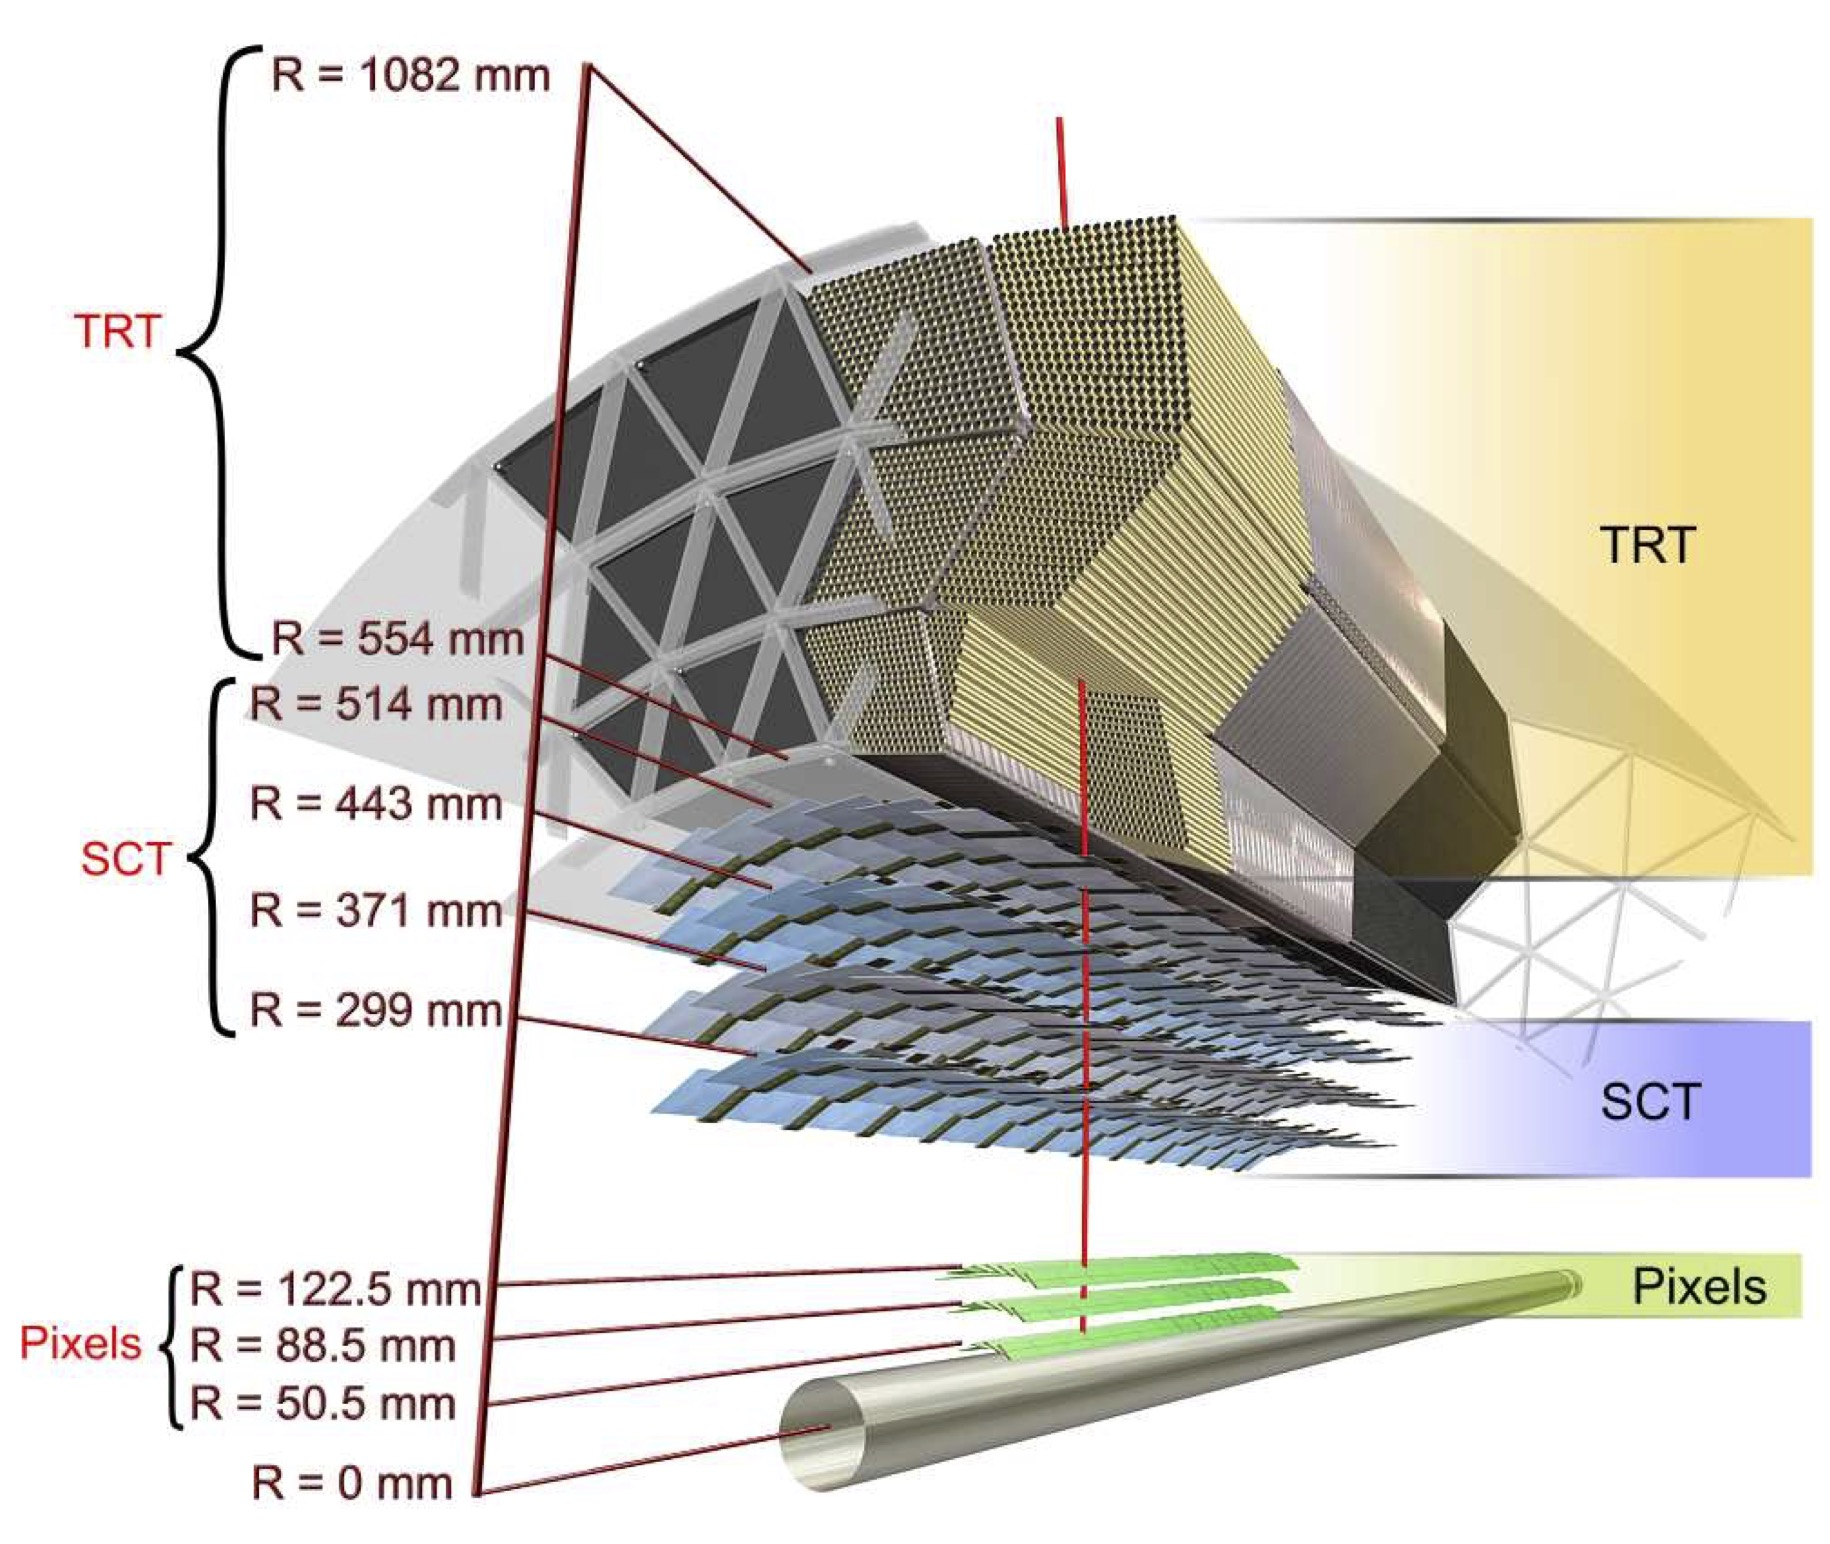
\includegraphics[width=9cm]{Chapters/CH2/figures/ID}
	\caption{Schematic view of the barrel of the ATLAS inner tracking system~\cite{ATLAS}.}
	\label{fig:ID}
\end{figure}
\\The ID is contained in a cylinder, 7 m long and 1.15 m in radius, placed in a 2 T solenoid magnetic field and it is designed to trace charged particles with a minimum moment of 0.1 GeV/c, it allows the measurement of the moment through the track curvature radius and the reconstruction of the main interaction and decay vertices (both primary and secondary).\\
The innermost part of the ID, which has a radius of about 15 cm, consists of silicon pixels to maximize the precision in the reconstruction of the tracks and the resistance to radiation.
The pixel detector records on average three points for each track, which allows a reconstruction of the secondary decay vertices. This detector has a total of approximately 80 million sensitive elements.
\vspace{\baselineskip}
\\The intermediate part, which covers a radius ranging from 30 to 60 cm, uses a microstrip detector (Semi-Conductor Tracker), to provide good spatial resolution.
The detection technique of the SCT relies on the same principle as for the pixel detector, however long strips are used compared to the rectangular pixels due to 
the smaller particle density in the outer layers.
It is located around the Pixel detector and is designed to provide eight precision measurements per track, contributing to the measurements of momentum, impact parameter and 
vertex position. The total number of sensitive items is around 6 million.
\vspace{\baselineskip}
\\The outermost layer ranges from 60 to 95 cm in radius; it is a gas detector (Transition Radiation Tracker) consisting of a set of small diameter tubes, containing $\mathrm{Xe}$ ($\mathrm{70\%}$), 
$\mathrm{CO_2}$ ($\mathrm{27\%}$),  $\mathrm{O_2}$ ($\mathrm{3\%}$); it provides a good resolution of the curvature of the track and contributes strongly to its reconstruction.\\\
The tracker contributes to the identification of the electrons, being sensitive to the emission of transition radiation that the particles emit when passing between different materials. 

\subsection{Calorimetric System}
\label{sec:CAL}
Calorimeters must provide good containment for electromagnetic and hadronic showers, they must limit punch-through into the muon system, and finally they must detect the particles that do not lose energy by ionization and are therefore not seen by the internal detector.\\
It is important that calorimeters cover the largest possible portion of solid angle; in fact, if a particle passes through a region without instrumentation, it is not detected and its energy contributes to the \textit{Missing Transverse Energy} (MET), the precision of which is essential for identifying and studying weakly interacting particles such as neutrinos and, possibly, new BSM particles. \\
In ATLAS there are two calorimeters: the Electromagnetic Calorimeter (ECAL)  and the Hadron Calorimeter (HCAL), as depicted in Figure~\ref{fig:cal} and they cover the range $\mathrm{|\eta|<4.9}$.  
\begin{figure}[h]
	\centering
	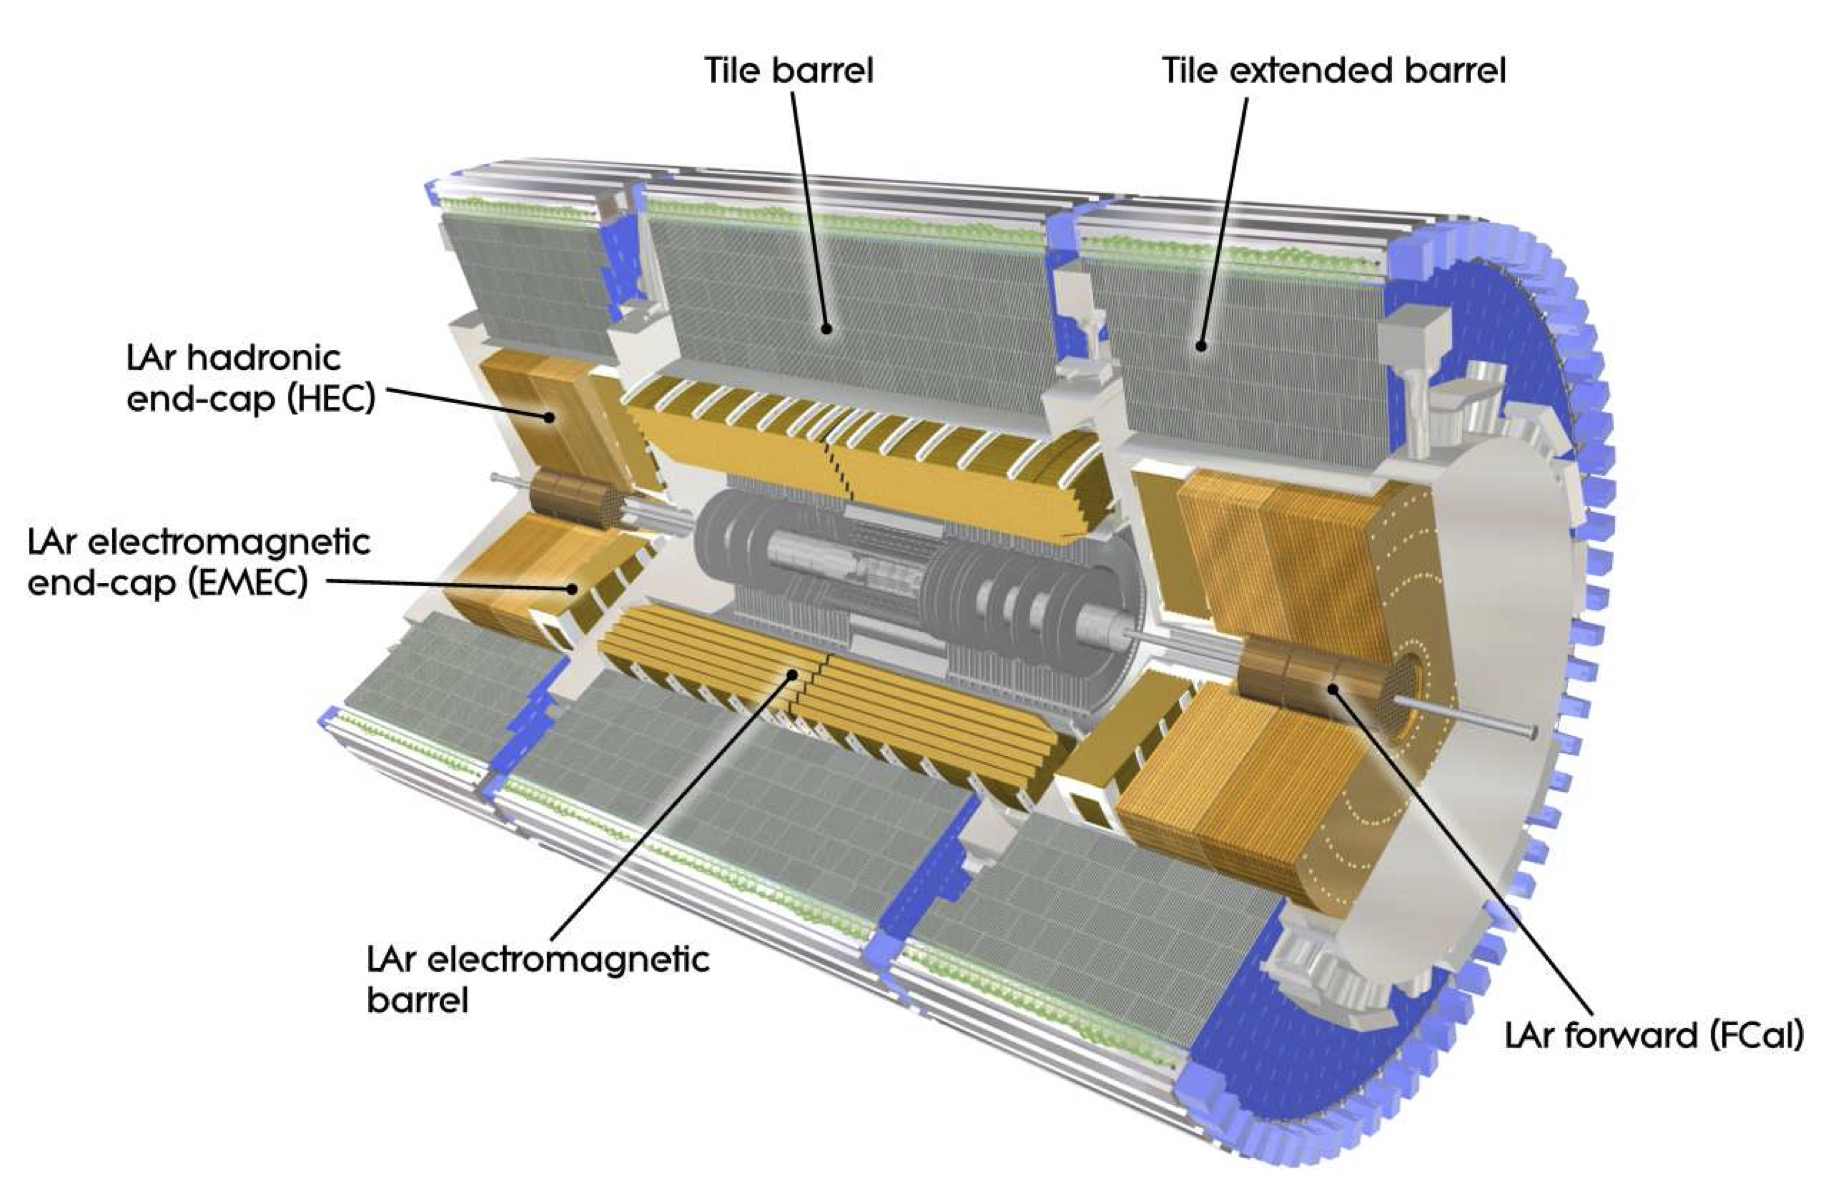
\includegraphics[width=10cm]{Chapters/CH2/figures/cal}
	\caption{Cut-away view of the ATLAS calorimeter system~\cite{ATLAS}.}
	\label{fig:cal}
\end{figure}
\vspace{\baselineskip}
\\The ECAL is divided into a barrel part ($\mathrm{|\eta|<1.475}$) and two end-cap components ($\mathrm{1.375<|\eta|<3.2}$), each housed in their own cryostat.
It is a lead-LAr detector with accordion-shaped kapton electrodes and lead absorber plates over its full coverage. The accordion geometry provides complete $\phi$ symmetry without azimuthal cracks.
The lead thickness in the absorber plates has been optimized as a function of $\eta$ in terms of ECAL performance in energy resolution. 
\\A schematic representation of the ECAL in the barrel and its main construction parameters are shown in Figure~\ref{fig:ECAL}. 
\begin{figure}[h]
	\centering
	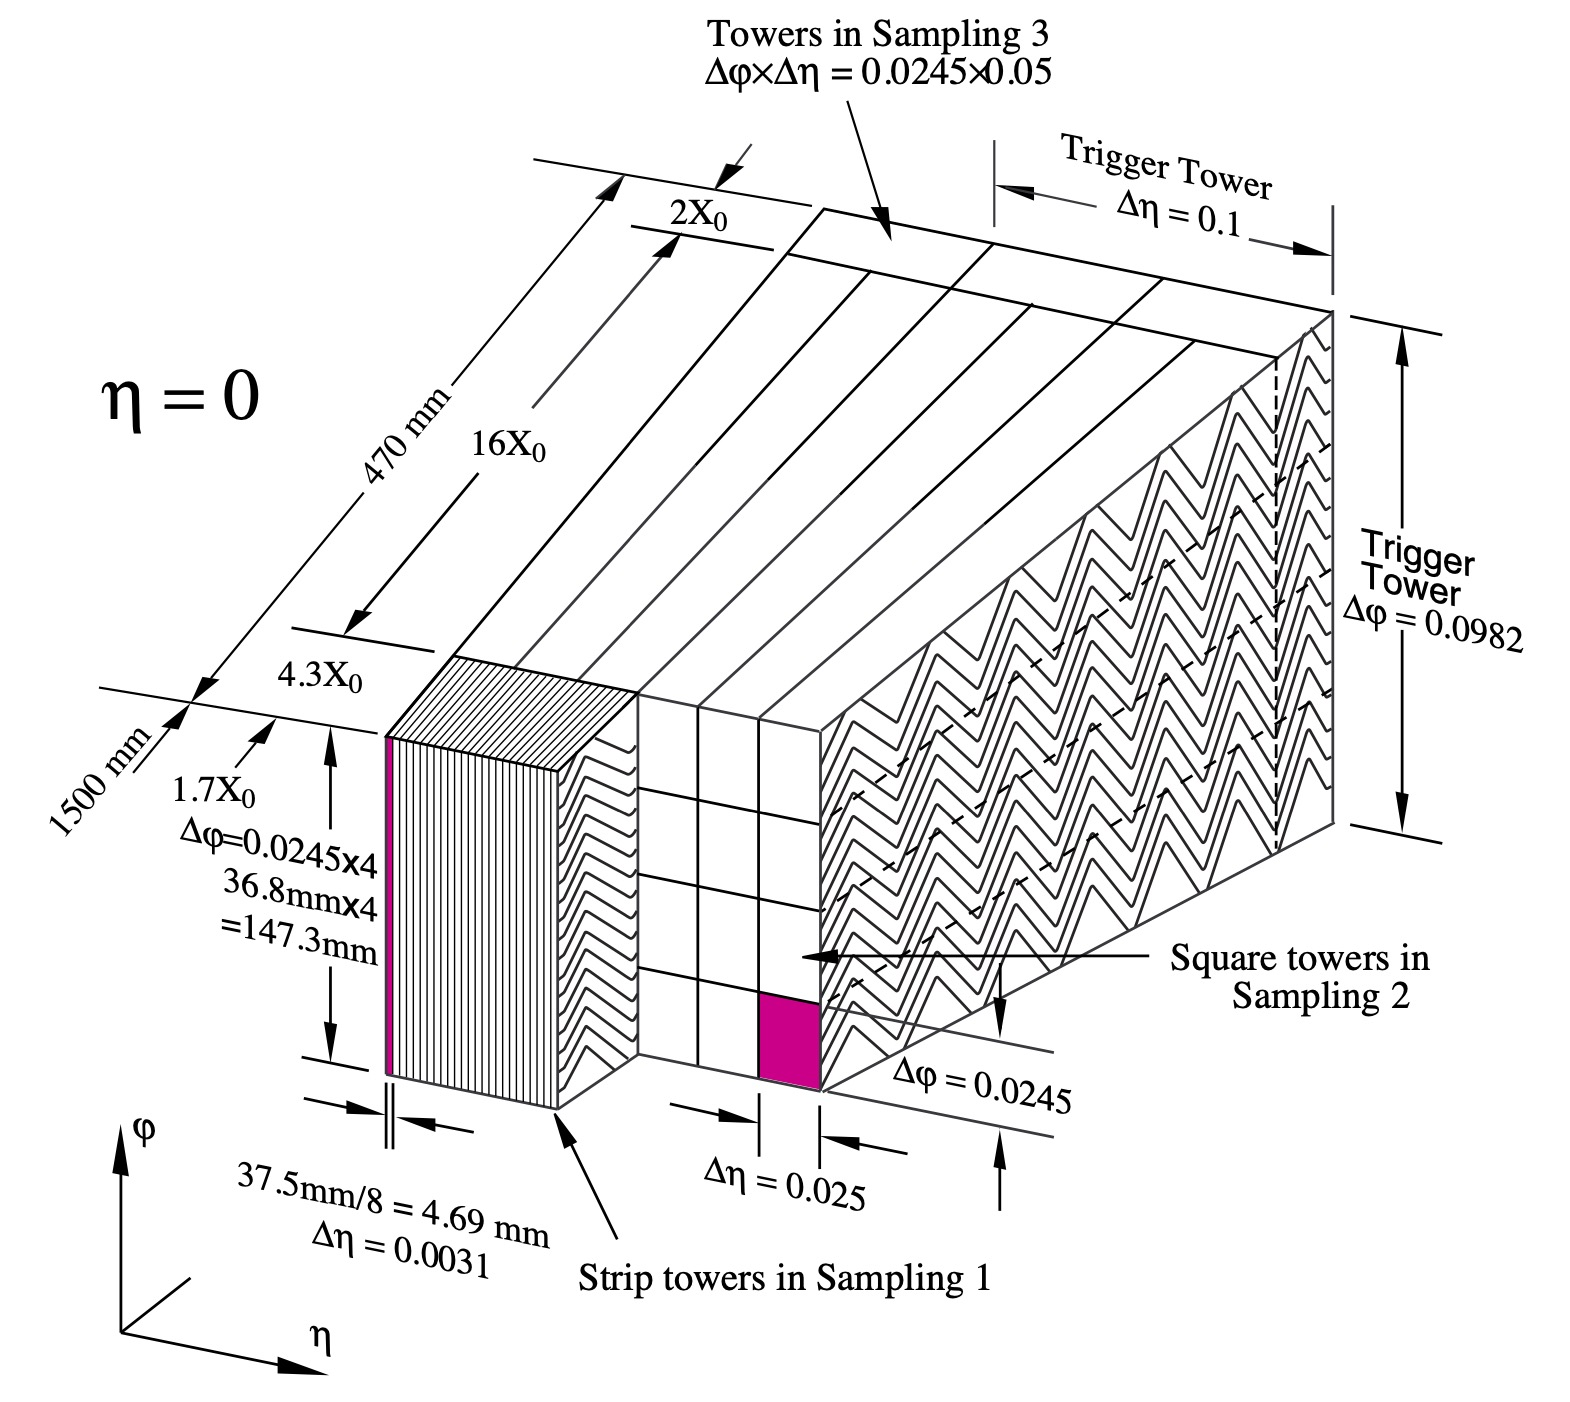
\includegraphics[width=7cm]{Chapters/CH2/figures/ECAL}
	\caption{Sketch of the accordion structure of the ECAL~\cite{cal}.}
	\label{fig:ECAL}
\end{figure}
\vspace{\baselineskip}
\\The outer calorimeter is the HCAL, which is divided in Tile Calorimeter (TileCal), the Hadronic End-cap Calorimeter (HEC) and the Forward Calorimeter (FCal). \\
LAr technology is also used for the hadronic calorimeters, matching the outer $|\eta|$ limits of end-cap electromagnetic calorimeters. 
The tile calorimeter barrel covers the region $\mathrm{|\eta|<1.0}$, and its two extended barrels the range $\mathrm{0.8<|\eta|<1.7}$, with a sampling calorimeter 
using steel as the absorber and scintillating tiles as the active material.\\
The HEC consists of two independent wheels per end-cap, located directly behind the end-cap electromagnetic calorimeter. The technology is similar to that of the 
electromagnetic calorimeter in the end-cap region, the active medium is LAr, but the absorption medium is made of copper rather than lead.
The FCal ($\mathrm{3.1<|\eta|<4.9}$) is integrated into the end-cap cryostats, as this provides clear benefits in terms of uniformity of the calorimetric coverage as well as reduced radiation background levels in 
the muon spectrometer. The FCal consists of three modules in each end-cap: the first, made of copper, is optimized for electromagnetic measurements, while the other two, made of tungsten, measure 
predominantly the energy of hadronic interactions.\\
An important quantity in calorimetry is the energy resolution, which is parameterized as:
\begin{equation}
\frac{\sigma_{E}}{E}=\frac{S}{\sqrt{E}} \oplus \frac{N}{E} \oplus C
\end{equation}
The first term represent the stochastic contribution related to the shower evolution, the second term
is related to the read-out electronics and the effect of the pile-up. The last term is a costant, due to systematic effects (e.g. mis-calibrations, dead detector material). 
The dominant source of uncertainty is linked, at low energy, with the high pile-up whereas, at high energy, C becomes the leading uncertainty. 

\FloatBarrier
\subsection{Muon Spectrometer}
\label{sec:MuonSpec}
The calorimeter is surrounded by the Muon Spectrometer (MS) depicted in Figure~\ref{fig:MS}, which is placed at the outermost part of the ATLAS detector.\\
The outer layers are reached by a few types of particles, mainly muons and neutrinos.\\
These muons ionize  in the material passed through, but the energy, lost in the electromagnetic interaction
with other nuclei of the calorimeter, is not sufficient to stop them. 
The MS  identifies muons and measures their momentum.
\begin{figure}[h]
	\centering
	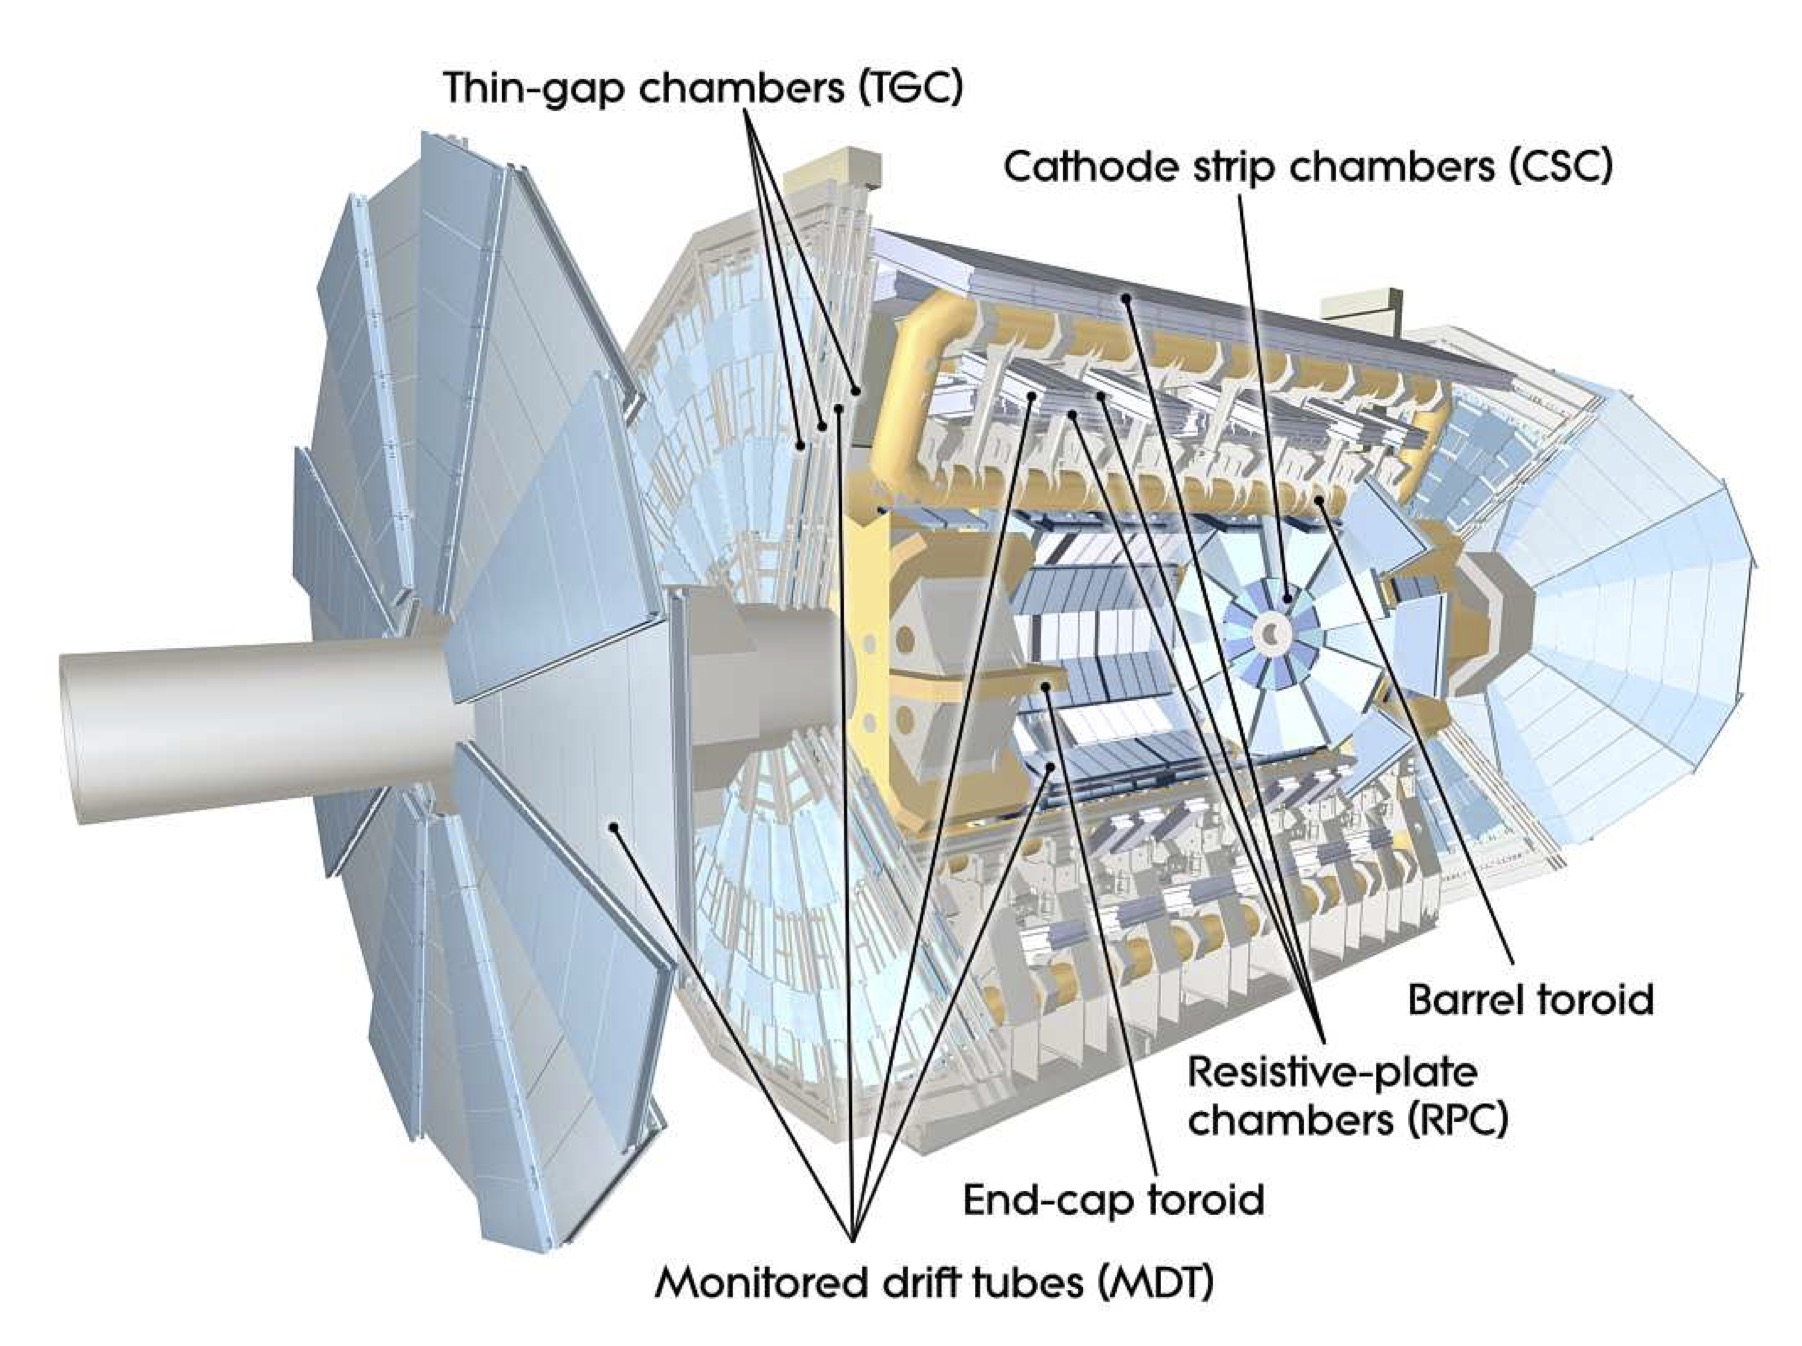
\includegraphics[width=10cm]{Chapters/CH2/figures/MS}
	\caption{Cut-away view of the ATLAS muon system~\cite{ATLAS}.}
	\label{fig:MS}
\end{figure}
\\A series of magnets arranged externally to the calorimeter creates a toroidal-shaped magnetic field that modifies the charged particles direction allowing the measurement of the momentum.
For muons with $\mathrm{p_T}$ > 30 GeV the measurement is much more precise than the measurement obtained by the inner detectors. 
For lower $\mathrm{p_T}$, on the other hand, the measurement is less accurate, due to the 
energy loss in the previous layers of the detector and taken in to account to handle \textit{soft muons}, presented in Section~\ref{sec:soft_muons}.\\
For both the central part and the end-caps,  there are two types of muon detectors:
\begin{itemize}
	\item a trigger system based on cameras with fast response, such as the \textit{Resistive Plate Chamber} (RPC) and the \textit{Thin Gap Chamber} (TGC), 
	\item precision tracking chambers, such as the \textit{Monitored Drift Tube} (MDT) and the \textit{Cathode Strip Chamber} (CGS).
\end{itemize}
\vspace{\baselineskip}
In the central region ($\mathrm {|\eta | <1.05}$), the RPCs consist of two parallel planes filled with a mixture of gas that ionizes when a muon passes through.
The HV applied between the plates allows the development of avalanches, along the ionization track towards the anode, which constitutes a signal.\\
In the end-cap ($\mathrm {1.05<|\eta |<2.4}$), TGCs are used to complement the RPCs in the triggering system for their good time resolution and rate capability. 
\\The TGC is a multi-wire proportional chamber operated in a highly quenching gas mixture.
Both TGCs and RPCs can achieve a read-out time of less than $\mathrm {25}$ ns~\cite{MS}.
\vspace{\baselineskip}
\\The MDTs are used for muons with $\mathrm {|\eta | <2}$, and they are a series of aluminium tubes filled with a gas mixture of Argon and $\mathrm {CO_2}$.
A central wire serving as anode allows to collect the electrons that are formed following the passage of the muon into the gas.
\\The CSCs cover the area while $ \mathrm {2 <| \eta | <2.7}$, and are radially-oriented proportional multi-wire chambers, i.e. metal chambers containing a system of parallel and perpendicular 
anodic wires with strips of opposite polarity.
\vspace{\baselineskip}
\\One important point to stress is that this detector measures the characteristics of any charged particle that passes through it and not just muons.
For this reason it is possible that other particles that are not muons, such as pions that manage to overcome the calorimeter are detected as muons.\\
%An estimation of fake soft muons rate is discussed in the Section~\ref{sec:fakeSMT}.
What is presented in this paragraph about the MS is a general overview but much more will be presented in Chapter~\ref{chapter:upgrade}, going deeper on its functioning
and its upgrade for the HL-LHC.

\FloatBarrier
\subsection{Trigger and Data Acquisition}
\label{sec:TrigSys}
Once fully operational, with the high frequency of collisions typical at LHC, an impressive amount of data is produced (40 MHz of p-p bunch collision frequency), 
which would be impossible to manage without the application of filters.
The \textit{Trigger and Data Acquisition system} (TDAQ) is able to recognize the interesting events for further study.\\
In Run2 the trigger system consists of two levels of event selection: the \textit{Level-1 trigger} (L1), is an hardware trigger that reduces the rate to 100 kHz, while the 
\textit{High-Level Trigger} (HLT), is a software trigger, further the reducing event rate to 1 kHz.\\
The Level-1 trigger is composed by three subsystems: 
the first is the L1 calorimeter trigger (L1Calo), which uses calorimeter information; 
the second is the L1 muon trigger (L1Muon), which primarily uses TGC and RPC information to make fast decisions on muon items; 
the third is the L1 topological trigger (L1Topo) that combines information from L1Calo and L1Muon into the Central Trigger Processor (CTP) which makes the final decision.\\
At this point, L1 identifies the \textit{Region of Interest} (RoI) with an event rate reduced  below 100 kHz.
The RoI are then used by the HLT, which has access to the information of all the sub-detectors, targeting the maximum rate of 1 kHz.\\
Finally, the events are assembled into an event record passes to the offline storage facilities for a complete off-line reconstruction~\cite{TrigSys}.





